\clearpage
%%%%%%%%%%%%%%%%%%%%%%%%%%%%%%%%%%%%%%%
\section{Modeling Cross checks} \label{modeling_xchecks}

In order to test the applicability of the statistical (signal and background) modeling proposed in this study, a cross-check procedure is performed by generating a set of pseudo-experiemnts (toys datasets) based on the  the signal plus background model, for each decay channel ($H/Z \rightarrow \Upsilon(1S,2S,3S,)+\gamma$) with some signal injected.

The procedure consists of resample from the signal plus background a number of events, including some extra (injected signal). The amount of injected signal is controlled by the $\mu_{true}$ variable, where $\mu_{true} = X$ means inject $X$ times the expected signal.

Once generated, the toy dataset is refitted to the signal plus background model and the signal strength ($\mu_{fit}$) and its error $\sigma_{fit}$ are extracted. This procedures is repeated 10000 times and only for the inclusive category. Figures~\ref{fig:fits_xchecks_mHZ_Z}, ~\ref{fig:fits_xchecks_mMuMNU_Z}, ~\ref{fig:fits_xchecks_mHZ_H} and \ref{fig:fits_xchecks_mMuMNU_H} show examples of those fits for the Higgs and Z decay.


\begin{figure}[!htbp]
\begin{center}
 %mu = 20
 \includegraphics[width=0.3\textwidth]{figures/modeling_xchecks/plots/ZToUpsilon1SPhoton_Cat0_signalStrenght_20/Cat0_mMuMNU_fit_s}
\includegraphics[width=0.3\textwidth]{figures/modeling_xchecks/plots/ZToUpsilon2SPhoton_Cat0_signalStrenght_20/Cat0_mMuMNU_fit_s}
\includegraphics[width=0.3\textwidth]{figures/modeling_xchecks/plots/ZToUpsilon3SPhoton_Cat0_signalStrenght_20/Cat0_mMuMNU_fit_s}
 %mu = 50
\includegraphics[width=0.3\textwidth]{figures/modeling_xchecks/plots/ZToUpsilon1SPhoton_Cat0_signalStrenght_50/Cat0_mMuMNU_fit_s}
\includegraphics[width=0.3\textwidth]{figures/modeling_xchecks/plots/ZToUpsilon2SPhoton_Cat0_signalStrenght_50/Cat0_mMuMNU_fit_s}
\includegraphics[width=0.3\textwidth]{figures/modeling_xchecks/plots/ZToUpsilon3SPhoton_Cat0_signalStrenght_50/Cat0_mMuMNU_fit_s}
 %mu = 100
\includegraphics[width=0.3\textwidth]{figures/modeling_xchecks/plots/ZToUpsilon1SPhoton_Cat0_signalStrenght_100/Cat0_mMuMNU_fit_s}
\includegraphics[width=0.3\textwidth]{figures/modeling_xchecks/plots/ZToUpsilon2SPhoton_Cat0_signalStrenght_100/Cat0_mMuMNU_fit_s}
\includegraphics[width=0.3\textwidth]{figures/modeling_xchecks/plots/ZToUpsilon3SPhoton_Cat0_signalStrenght_100/Cat0_mMuMNU_fit_s}
 %mu = 1000
\includegraphics[width=0.3\textwidth]{figures/modeling_xchecks/plots/ZToUpsilon1SPhoton_Cat0_signalStrenght_1000/Cat0_mMuMNU_fit_s}
\includegraphics[width=0.3\textwidth]{figures/modeling_xchecks/plots/ZToUpsilon2SPhoton_Cat0_signalStrenght_1000/Cat0_mMuMNU_fit_s}
\includegraphics[width=0.3\textwidth]{figures/modeling_xchecks/plots/ZToUpsilon3SPhoton_Cat0_signalStrenght_1000/Cat0_mMuMNU_fit_s}
\end{center}
\caption{Examples of the toy datasets fit ($M_{\mu\mu}$), for the Z decay analysis, after the toy dataset refit, for 1S, 2S and 3S (left to right), with $\mu_{true}$ equals to 20, 50, 100, 1000 (top to bottom). The red lines corresponds to the background model (B), the green lines to signal model (S), the blue lines to the total (S+B) and the dots is the toy dataset.}
\label{fig:fits_xchecks_mMuMNU_Z}
\end{figure}



\begin{figure}[!htbp]
\begin{center}
 %mu = 20
 \includegraphics[width=0.3\textwidth]{figures/modeling_xchecks/plots/ZToUpsilon1SPhoton_Cat0_signalStrenght_20/Cat0_mHZ_fit_s}
\includegraphics[width=0.3\textwidth]{figures/modeling_xchecks/plots/ZToUpsilon2SPhoton_Cat0_signalStrenght_20/Cat0_mHZ_fit_s}
\includegraphics[width=0.3\textwidth]{figures/modeling_xchecks/plots/ZToUpsilon3SPhoton_Cat0_signalStrenght_20/Cat0_mHZ_fit_s}
 %mu = 50
\includegraphics[width=0.3\textwidth]{figures/modeling_xchecks/plots/ZToUpsilon1SPhoton_Cat0_signalStrenght_50/Cat0_mHZ_fit_s}
\includegraphics[width=0.3\textwidth]{figures/modeling_xchecks/plots/ZToUpsilon2SPhoton_Cat0_signalStrenght_50/Cat0_mHZ_fit_s}
\includegraphics[width=0.3\textwidth]{figures/modeling_xchecks/plots/ZToUpsilon3SPhoton_Cat0_signalStrenght_50/Cat0_mHZ_fit_s}
 %mu = 100
\includegraphics[width=0.3\textwidth]{figures/modeling_xchecks/plots/ZToUpsilon1SPhoton_Cat0_signalStrenght_100/Cat0_mHZ_fit_s}
\includegraphics[width=0.3\textwidth]{figures/modeling_xchecks/plots/ZToUpsilon2SPhoton_Cat0_signalStrenght_100/Cat0_mHZ_fit_s}
\includegraphics[width=0.3\textwidth]{figures/modeling_xchecks/plots/ZToUpsilon3SPhoton_Cat0_signalStrenght_100/Cat0_mHZ_fit_s}
 %mu = 1000
\includegraphics[width=0.3\textwidth]{figures/modeling_xchecks/plots/ZToUpsilon1SPhoton_Cat0_signalStrenght_1000/Cat0_mHZ_fit_s}
\includegraphics[width=0.3\textwidth]{figures/modeling_xchecks/plots/ZToUpsilon2SPhoton_Cat0_signalStrenght_1000/Cat0_mHZ_fit_s}
\includegraphics[width=0.3\textwidth]{figures/modeling_xchecks/plots/ZToUpsilon3SPhoton_Cat0_signalStrenght_1000/Cat0_mHZ_fit_s}
\end{center}
\caption{Examples of the toy datasets fit ($M_{\mu\mu\gamma}$), for the Z decay analysis, after the toy dataset refit, for 1S, 2S and 3S (left to right), with $\mu_{true}$ equals to 20, 50, 100, 1000 (top to bottom). The red lines corresponds to the background model (B), the green lines to signal model (S), the blue lines to the total (S+B) and the dots is the toy dataset.}
\label{fig:fits_xchecks_mHZ_Z}
\end{figure}



\begin{figure}[!htbp]
\begin{center}
 %mu = 20
 \includegraphics[width=0.3\textwidth]{figures/modeling_xchecks/plots/HToUpsilon1SPhoton_Cat0_signalStrenght_100000/Cat0_mMuMNU_fit_s}
\includegraphics[width=0.3\textwidth]{figures/modeling_xchecks/plots/HToUpsilon2SPhoton_Cat0_signalStrenght_100000/Cat0_mMuMNU_fit_s}
\includegraphics[width=0.3\textwidth]{figures/modeling_xchecks/plots/HToUpsilon3SPhoton_Cat0_signalStrenght_100000/Cat0_mMuMNU_fit_s}
\includegraphics[width=0.3\textwidth]{figures/modeling_xchecks/plots/HToUpsilon1SPhoton_Cat0_signalStrenght_200000/Cat0_mMuMNU_fit_s}
\includegraphics[width=0.3\textwidth]{figures/modeling_xchecks/plots/HToUpsilon2SPhoton_Cat0_signalStrenght_200000/Cat0_mMuMNU_fit_s}
\includegraphics[width=0.3\textwidth]{figures/modeling_xchecks/plots/HToUpsilon3SPhoton_Cat0_signalStrenght_200000/Cat0_mMuMNU_fit_s}
\includegraphics[width=0.3\textwidth]{figures/modeling_xchecks/plots/HToUpsilon1SPhoton_Cat0_signalStrenght_300000/Cat0_mMuMNU_fit_s}
\includegraphics[width=0.3\textwidth]{figures/modeling_xchecks/plots/HToUpsilon2SPhoton_Cat0_signalStrenght_300000/Cat0_mMuMNU_fit_s}
\includegraphics[width=0.3\textwidth]{figures/modeling_xchecks/plots/HToUpsilon3SPhoton_Cat0_signalStrenght_300000/Cat0_mMuMNU_fit_s}
\includegraphics[width=0.3\textwidth]{figures/modeling_xchecks/plots/HToUpsilon1SPhoton_Cat0_signalStrenght_1000000/Cat0_mMuMNU_fit_s}
\includegraphics[width=0.3\textwidth]{figures/modeling_xchecks/plots/HToUpsilon2SPhoton_Cat0_signalStrenght_1000000/Cat0_mMuMNU_fit_s}
\includegraphics[width=0.3\textwidth]{figures/modeling_xchecks/plots/HToUpsilon3SPhoton_Cat0_signalStrenght_1000000/Cat0_mMuMNU_fit_s}
\end{center}
\caption{Examples of the toy datasets fit ($M_{\mu\mu}$), for the Higgs decay analysis, after the toy dataset refit, for 1S, 2S and 3S (left to right), with $\mu_{true}$ equals to 100000, 200000, 300000, 1000000 (top to bottom). The red lines corresponds to the background model (B), the green lines to signal model (S), the blue lines to the total (S+B) and the dots is the toy dataset.}
\label{fig:fits_xchecks_mMuMNU_H}
\end{figure}





\begin{figure}[!htbp]
\begin{center}
 \includegraphics[width=0.3\textwidth]{figures/modeling_xchecks/plots/HToUpsilon1SPhoton_Cat0_signalStrenght_100000/Cat0_mHZ_fit_s}
\includegraphics[width=0.3\textwidth]{figures/modeling_xchecks/plots/HToUpsilon2SPhoton_Cat0_signalStrenght_100000/Cat0_mHZ_fit_s}
\includegraphics[width=0.3\textwidth]{figures/modeling_xchecks/plots/HToUpsilon3SPhoton_Cat0_signalStrenght_100000/Cat0_mHZ_fit_s}
\includegraphics[width=0.3\textwidth]{figures/modeling_xchecks/plots/HToUpsilon1SPhoton_Cat0_signalStrenght_200000/Cat0_mHZ_fit_s}
\includegraphics[width=0.3\textwidth]{figures/modeling_xchecks/plots/HToUpsilon2SPhoton_Cat0_signalStrenght_200000/Cat0_mHZ_fit_s}
\includegraphics[width=0.3\textwidth]{figures/modeling_xchecks/plots/HToUpsilon3SPhoton_Cat0_signalStrenght_200000/Cat0_mHZ_fit_s}
\includegraphics[width=0.3\textwidth]{figures/modeling_xchecks/plots/HToUpsilon1SPhoton_Cat0_signalStrenght_300000/Cat0_mHZ_fit_s}
\includegraphics[width=0.3\textwidth]{figures/modeling_xchecks/plots/HToUpsilon2SPhoton_Cat0_signalStrenght_300000/Cat0_mHZ_fit_s}
\includegraphics[width=0.3\textwidth]{figures/modeling_xchecks/plots/HToUpsilon3SPhoton_Cat0_signalStrenght_300000/Cat0_mHZ_fit_s}
\includegraphics[width=0.3\textwidth]{figures/modeling_xchecks/plots/HToUpsilon1SPhoton_Cat0_signalStrenght_1000000/Cat0_mHZ_fit_s}
\includegraphics[width=0.3\textwidth]{figures/modeling_xchecks/plots/HToUpsilon2SPhoton_Cat0_signalStrenght_1000000/Cat0_mHZ_fit_s}
\includegraphics[width=0.3\textwidth]{figures/modeling_xchecks/plots/HToUpsilon3SPhoton_Cat0_signalStrenght_1000000/Cat0_mHZ_fit_s}
\end{center}
\caption{Examples of the toy datasets fit ($M_{\mu\mu\gamma}$), for the Higgs decay analysis, after the toy dataset refit, for 1S, 2S and 3S (left to right), with $\mu_{true}$ equals to 100000, 200000, 300000, 1000000 (top to bottom). The red lines corresponds to the background model (B), the green lines to signal model (S), the blue lines to the total (S+B) and the dots is the toy dataset.}
\label{fig:fits_xchecks_mHZ_H}
\end{figure}








It is expected that the pulls distribution for the fitted signal strength ($\frac{\mu_{fit} - \mu_{true}}{\sigma_{fit}}$) should follow a Gaussian distribution centered in 0 and with $\sigma$ around 1. Figures~\ref{fig:modeling_xchecks_Z} and \ref{fig:modeling_xchecks_H} present those pulls distributions for the Z and Higgs decays, respectively.






\begin{figure}[!htbp]
\begin{center}
 %mu = 20
 \includegraphics[width=0.3\textwidth]{figures/modeling_xchecks/plots/ZToUpsilon1SPhoton_Cat0_signalStrenght_20/pulls}
\includegraphics[width=0.3\textwidth]{figures/modeling_xchecks/plots/ZToUpsilon2SPhoton_Cat0_signalStrenght_20/pulls}
\includegraphics[width=0.3\textwidth]{figures/modeling_xchecks/plots/ZToUpsilon3SPhoton_Cat0_signalStrenght_20/pulls}
 %mu = 50
\includegraphics[width=0.3\textwidth]{figures/modeling_xchecks/plots/ZToUpsilon1SPhoton_Cat0_signalStrenght_50/pulls}
\includegraphics[width=0.3\textwidth]{figures/modeling_xchecks/plots/ZToUpsilon2SPhoton_Cat0_signalStrenght_50/pulls}
\includegraphics[width=0.3\textwidth]{figures/modeling_xchecks/plots/ZToUpsilon3SPhoton_Cat0_signalStrenght_50/pulls}
 %mu = 100
\includegraphics[width=0.3\textwidth]{figures/modeling_xchecks/plots/ZToUpsilon1SPhoton_Cat0_signalStrenght_100/pulls}
\includegraphics[width=0.3\textwidth]{figures/modeling_xchecks/plots/ZToUpsilon2SPhoton_Cat0_signalStrenght_100/pulls}
\includegraphics[width=0.3\textwidth]{figures/modeling_xchecks/plots/ZToUpsilon3SPhoton_Cat0_signalStrenght_100/pulls}
 %mu = 1000
\includegraphics[width=0.3\textwidth]{figures/modeling_xchecks/plots/ZToUpsilon1SPhoton_Cat0_signalStrenght_1000/pulls}
\includegraphics[width=0.3\textwidth]{figures/modeling_xchecks/plots/ZToUpsilon2SPhoton_Cat0_signalStrenght_1000/pulls}
\includegraphics[width=0.3\textwidth]{figures/modeling_xchecks/plots/ZToUpsilon3SPhoton_Cat0_signalStrenght_1000/pulls}
\end{center}
\caption{Distribution of pulls ($\frac{\mu_{fit} - \mu_{true}}{\sigma_{fit}}$), for the Z decay analysis, after the toy dataset refit, for 1S, 2S and 3S (left to right), with $\mu_{true}$ equals to 20, 50, 100, 1000 (top to bottom).}
\label{fig:modeling_xchecks_Z}
\end{figure}




\begin{figure}[!htbp]
\begin{center}
\includegraphics[width=0.3\textwidth]{figures/modeling_xchecks/plots/HToUpsilon1SPhoton_Cat0_signalStrenght_100000/pulls}
\includegraphics[width=0.3\textwidth]{figures/modeling_xchecks/plots/HToUpsilon2SPhoton_Cat0_signalStrenght_100000/pulls}
\includegraphics[width=0.3\textwidth]{figures/modeling_xchecks/plots/HToUpsilon3SPhoton_Cat0_signalStrenght_100000/pulls}
\includegraphics[width=0.3\textwidth]{figures/modeling_xchecks/plots/HToUpsilon1SPhoton_Cat0_signalStrenght_200000/pulls}
\includegraphics[width=0.3\textwidth]{figures/modeling_xchecks/plots/HToUpsilon2SPhoton_Cat0_signalStrenght_200000/pulls}
\includegraphics[width=0.3\textwidth]{figures/modeling_xchecks/plots/HToUpsilon3SPhoton_Cat0_signalStrenght_200000/pulls}
\includegraphics[width=0.3\textwidth]{figures/modeling_xchecks/plots/HToUpsilon1SPhoton_Cat0_signalStrenght_300000/pulls}
\includegraphics[width=0.3\textwidth]{figures/modeling_xchecks/plots/HToUpsilon2SPhoton_Cat0_signalStrenght_300000/pulls}
\includegraphics[width=0.3\textwidth]{figures/modeling_xchecks/plots/HToUpsilon3SPhoton_Cat0_signalStrenght_300000/pulls}
\includegraphics[width=0.3\textwidth]{figures/modeling_xchecks/plots/HToUpsilon1SPhoton_Cat0_signalStrenght_1000000/pulls}
\includegraphics[width=0.3\textwidth]{figures/modeling_xchecks/plots/HToUpsilon2SPhoton_Cat0_signalStrenght_1000000/pulls}
\includegraphics[width=0.3\textwidth]{figures/modeling_xchecks/plots/HToUpsilon3SPhoton_Cat0_signalStrenght_1000000/pulls}
\end{center}
\caption{Distribution of pulls ($\frac{\mu_{fit} - \mu_{true}}{\sigma_{fit}}$), for the Higgs decay analysis, after the toy dataset refit, for 1S, 2S and 3S (left to right), with $\mu_{true}$ equals to 100000, 200000, 300000, 1000000 (top to bottom).}
\label{fig:modeling_xchecks_H}
\end{figure}


As a general conclusion on this cross check, as long as the toy MC generation is able to inject enough signal to be fit, the final modeling of this analysis is able to recover a Gaussian pulls distribution. This, of course, depends on the $\Upsilon$ state to be considered. For the Z decay, between $\mu_{true} = 50$ and  $\mu_{true} = 100$ (around a hundred of events passing full selection), while for the Higgs decay, it is needed only a few events after full selection, even thought it means hundreds of thousands times the expected signal, since the very small cross sections for the decay, as shown in Table~\ref{tab:MC}.

\clearpage

